%%%% Paramétrage du cours %%%%
\def\xxactivite{Cours}
\def\xxauteur{\textsl{Xavier Pessoles}}

\fichefalse
\proftrue
\tdfalse
\courstrue

\def\xxnumchapitre{Chapitre 1 \vspace{.2cm}}
\def\xxchapitre{\hspace{.12cm} Détermination des liaisons équivalentes}

\def\xxcompetences{%
\textsl{%
\textbf{Savoirs et compétences :}\\
\begin{itemize}[label=\ding{112},font=\color{ocre}] 
\item B2-12 : proposer un modèle cinématique à partir d'un système réel ou d'une maquette numérique.
;
\item B2-15 : Simplifier un modèle de mécanisme.
\end{itemize}
}}


\def\xxfigures{
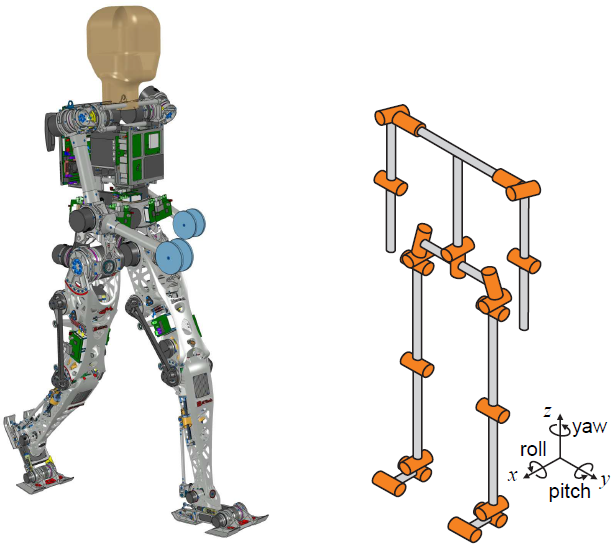
\includegraphics[width=0.6\textwidth]{lola}\\
\textit{Robot humanoïde Lola}

\vspace{.5cm}

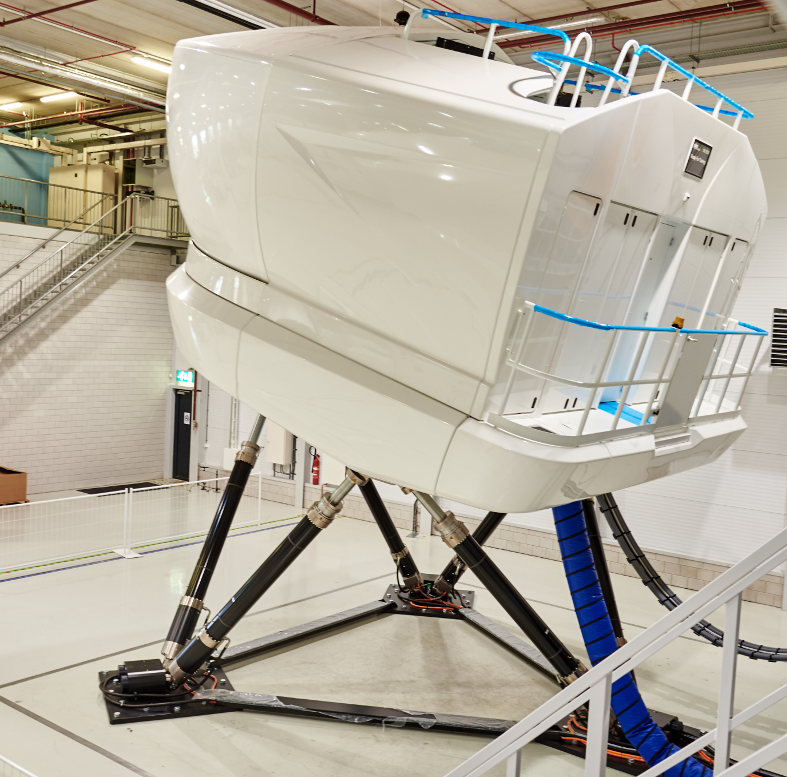
\includegraphics[width=0.5\textwidth]{simu}\\
\textit{Simulateur de vol Lockheed Martin}
}%figues de la page de garde%figues de la page de garde

\pagestyle{empty}


%%%%%%%% PAGE DE GARDE COURS
\ifcours
\begin{tikzpicture}[remember picture,overlay]
\node at (current page.north west)
{\begin{tikzpicture}[remember picture,overlay]
\node[anchor=north west,inner sep=0pt] at (0,0) {\includegraphics[width=\paperwidth]{\thechapterimage}};
\draw[anchor=west] (-2cm,-8cm) node [line width=2pt,rounded corners=15pt,draw=ocre,fill=white,fill opacity=0.6,inner sep=40pt]{\strut\makebox[22cm]{}};
\draw[anchor=west] (1cm,-8cm) node {\huge\sffamily\bfseries\color{black} %
\begin{minipage}{1cm}
\rotatebox{90}{\LARGE\sffamily\textsc{\color{ocre}\textbf{\xxnumpartie}}}
\end{minipage} \hfill
\begin{minipage}[c]{14cm}
\begin{titrepartie}
\begin{flushright}
\renewcommand{\baselinestretch}{1.1} 
\Large\sffamily\textsc{\textbf{\xxpartie}}
\renewcommand{\baselinestretch}{1} 
\end{flushright}
\end{titrepartie}
\end{minipage} \hfill
\begin{minipage}[c]{3.5cm}
{\large\sffamily\textsc{\textbf{\color{ocre} \discipline}}}
\end{minipage} 
 };
\end{tikzpicture}};
\end{tikzpicture}


\begin{tikzpicture}[overlay]
\node[shape=rectangle, 
      rounded corners = .25 cm,
	  draw= ocre,
	  line width=2pt, 
	  fill = ocre!10,
	  minimum width  = 2.5cm,
	  minimum height = 3cm,] at (18cm,0) {};
\node at (17.7cm,0) {\rotatebox{90}{\textbf{\Large\color{ocre}{\classe}}}};
%{};
\end{tikzpicture}

\vspace{3.5cm}

\begin{tikzpicture}[remember picture,overlay]
\draw[anchor=west] (-2cm,-6cm) node {\huge\sffamily\bfseries\color{black} %
\begin{minipage}{2cm}
\begin{center}
\LARGE\sffamily\textsc{\color{ocre}\textbf{\xxactivite}}
\end{center}
\end{minipage} \hfill
\begin{minipage}[c]{15cm}
\begin{titrechapitre}
\renewcommand{\baselinestretch}{1.1} 
\Large\sffamily\textsc{\textbf{\xxnumchapitre}}

\Large\sffamily\textsc{\textbf{\xxchapitre}}
\vspace{.5cm}

\renewcommand{\baselinestretch}{1} 
\normalsize\normalfont
\xxcompetences
\end{titrechapitre}
\end{minipage}  };
\end{tikzpicture}
\vfill

\begin{flushright}
\begin{minipage}[c]{.3\linewidth}
\begin{center}
\xxfigures
\end{center}
\end{minipage}\hfill
\begin{minipage}[c]{.6\linewidth}
\startcontents
\printcontents{}{1}{}
\end{minipage}
\end{flushright}

\begin{tikzpicture}[remember picture,overlay]
\draw[anchor=west] (4.5cm,-.7cm) node {
\begin{minipage}[c]{.2\linewidth}
\begin{flushright}

\includegraphics[width=2cm]{png/logoCC}
\end{flushright}
\end{minipage}
\begin{minipage}[c]{.2\linewidth}
\textsl{\xxauteur} \\
\textsl{\classe}
\end{minipage}
 };
\end{tikzpicture}
\newpage
\pagestyle{fancy}

\newpage
\pagestyle{fancy}

\else
\fi


%%%%%%%% PAGE DE GARDE TD
\iftd
%\begin{tikzpicture}[remember picture,overlay]
%\node at (current page.north west)
%{\begin{tikzpicture}[remember picture,overlay]
%\draw[anchor=west] (-2cm,-3.25cm) node [line width=2pt,rounded corners=15pt,draw=ocre,fill=white,fill opacity=0.6,inner sep=40pt]{\strut\makebox[22cm]{}};
%\draw[anchor=west] (1cm,-3.25cm) node {\huge\sffamily\bfseries\color{black} %
%\begin{minipage}{1cm}
%\rotatebox{90}{\LARGE\sffamily\textsc{\color{ocre}\textbf{\xxnumpartie}}}
%\end{minipage} \hfill
%\begin{minipage}[c]{13.5cm}
%\begin{titrepartie}
%\begin{flushright}
%\renewcommand{\baselinestretch}{1.1} 
%\Large\sffamily\textsc{\textbf{\xxpartie}}
%\renewcommand{\baselinestretch}{1} 
%\end{flushright}
%\end{titrepartie}
%\end{minipage} \hfill
%\begin{minipage}[c]{3.5cm}
%{\large\sffamily\textsc{\textbf{\color{ocre} \discipline}}}
%\end{minipage} 
% };
%\end{tikzpicture}};
%\end{tikzpicture}

%%%%%%%%%% PAGE DE GARDE TD %%%%%%%%%%%%%%%
%\begin{tikzpicture}[overlay]
%\node[shape=rectangle, 
%      rounded corners = .25 cm,
%	  draw= ocre,
%	  line width=2pt, 
%	  fill = ocre!10,
%	  minimum width  = 2.5cm,
%	  minimum height = 2.5cm,] at (18.5cm,0) {};
%\node at (17.7cm,0) {\rotatebox{90}{\textbf{\Large\color{ocre}{\classe}}}};
%%{};
%\end{tikzpicture}

% PARTIE ET CHAPITRE
%\begin{tikzpicture}[remember picture,overlay]
%\draw[anchor=west] (-1cm,-2.1cm) node {\large\sffamily\bfseries\color{black} %
%\begin{minipage}[c]{15cm}
%\begin{flushleft}
%\xxnumchapitre \\
%\xxchapitre
%\end{flushleft}
%\end{minipage}  };
%\end{tikzpicture}

% Bandeau titre exo
\begin{tikzpicture}[remember picture,overlay]
\draw[anchor=west] (-2cm,-4cm) node {\huge\sffamily\bfseries\color{black} %
\begin{minipage}{5cm}
\begin{center}
\LARGE\sffamily\color{ocre}\textbf{\textsc{\xxactivite}}

\begin{center}
\xxfigures
\end{center}

\end{center}
\end{minipage} \hfill
\begin{minipage}[c]{12cm}
\begin{titrechapitre}
\renewcommand{\baselinestretch}{1.1} 
\large\sffamily\textbf{\textsc{\xxtitreexo}}

\small\sffamily{\textbf{\textit{\color{black!70}\xxsourceexo}}}
\vspace{.5cm}

\renewcommand{\baselinestretch}{1} 
\normalsize\normalfont
\xxcompetences
\end{titrechapitre}
\end{minipage}  };
\end{tikzpicture}

\else
\fi


%%%%%%%% PAGE DE GARDE FICHE
\iffiche
\begin{tikzpicture}[remember picture,overlay]
\node at (current page.north west)
{\begin{tikzpicture}[remember picture,overlay]
\draw[anchor=west] (-2cm,-3.25cm) node [line width=2pt,rounded corners=15pt,draw=ocre,fill=white,fill opacity=0.6,inner sep=40pt]{\strut\makebox[22cm]{}};
\draw[anchor=west] (1cm,-3.25cm) node {\huge\sffamily\bfseries\color{black} %
\begin{minipage}{1cm}
\rotatebox{90}{\LARGE\sffamily\textsc{\color{ocre}\textbf{\xxnumpartie}}}
\end{minipage} \hfill
\begin{minipage}[c]{14cm}
\begin{titrepartie}
\begin{flushright}
\renewcommand{\baselinestretch}{1.1} 
\large\sffamily\textsc{\textbf{\xxpartie} \\} 

\vspace{.2cm}

\normalsize\sffamily\textsc{\textbf{\xxnumchapitre -- \xxchapitre}}
\renewcommand{\baselinestretch}{1} 
\end{flushright}
\end{titrepartie}
\end{minipage} \hfill
\begin{minipage}[c]{3.5cm}
{\large\sffamily\textsc{\textbf{\color{ocre} \discipline}}}
\end{minipage} 
 };
\end{tikzpicture}};
\end{tikzpicture}


\begin{tikzpicture}[overlay]
\node[shape=rectangle, 
      rounded corners = .25 cm,
	  draw= ocre,
	  line width=2pt, 
	  fill = ocre!10,
	  minimum width  = 2.5cm,
	  minimum height = 2.5cm,] at (18.5cm,0.5cm) {};
%	  minimum height = 2.5cm,] at (18.5cm,0cm) {};
\node at (17.7cm,0.5) {\rotatebox{90}{\textsf{\textbf{\large\color{ocre}{\classe}}}}};
%{};
\end{tikzpicture}



\else
\fi



\vspace{2cm}
\pagestyle{fancy}
\thispagestyle{plain}


\section{Introduction}
\subsection{Rappel sur les torseurs des liaisons}
\begin{defi}
De manière générale, le torseur cinématique peut être noté :
$$
\torseurcin{V}{i}{j}
=\torseurl{\vecto{i}{j}}{\vectv{P}{i}{j}}{P}
=\torseurl{p_{ij}\vect{x}+q_{ij}\vect{y}+r_{ij}\vect{z}}{u_{ij}\vect{x}+v_{ij}\vect{y}+w_{ij}\vect{z}}{P}
=\torseurcol{p_{ij}}{q_{ij}}{r_{ij}}{u_{ij}}{v_{ij}}{w_{ij}}{P,\mathcal{R}}.
$$

\textbf{On notera $n_c$ le nombre d'inconnues cinématiques d'une liaison.} En d'autres termes, $n_c$ correspond donc au nombre de mobilités de la liaison.
\end{defi}

\begin{defi}
De manière générale, le torseur statique peut être noté :
$$
\torseurstat{T}{i}{j}
=\torseurl{\vectf{i}{j}}{\vectm{P}{i}{j}}{P}
=\torseurl{X_{ij}\vect{x}+Y_{ij}\vect{y}+Z_{ij}\vect{z}}{L_{ij}\vect{x}+M_{ij}\vect{y}+N_{ij}\vect{z}}{P}
=\torseurcol{X_{ij}}{Y_{ij}}{Z_{ij}}{L_{ij}}{M_{ij}}{N_{ij}}{P,\mathcal{R}}.
$$

\textbf{On notera $n_s$ le nombre d'inconnues statiques d'une liaison.} En d'autres termes, $n_s$ correspond au degré de liaison. On a $n_s=6-n_c$.
\end{defi}
\subsection{Graphe des liaisons}

\begin{defi}
Selon la forme du graphe de liaisons, on peut distinguer 3 cas :
\begin{multicols}{3}
\begin{center}
\textbf{Les chaînes ouvertes} 
\end{center}

\begin{center}
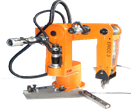
\includegraphics[width=.6\linewidth]{ericc_01}

\vspace{.5cm}

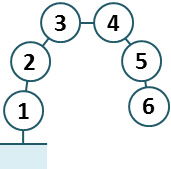
\includegraphics[width=.6\linewidth]{ericc_02}
\end{center}

\begin{center}
\textbf{Les chaînes fermées} 
\end{center}

\begin{center}
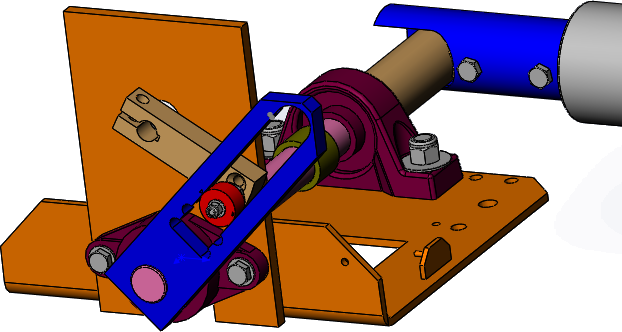
\includegraphics[width=.8\linewidth]{sympact_01}

\vspace{.5cm}

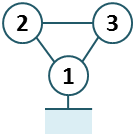
\includegraphics[width=.6\linewidth]{sympact_02}
\end{center}

\vfill\null
\columnbreak

\begin{center}
\textbf{Les chaînes complexes} 
\end{center}

\begin{center}

\includegraphics[width=.95\linewidth]{haptique_01}

\vspace{.5cm}

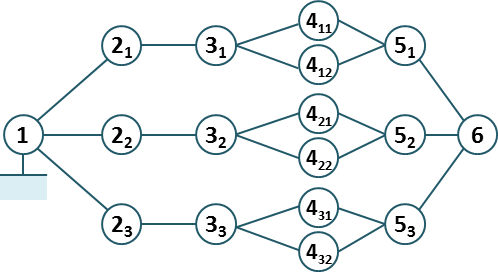
\includegraphics[width=.95\linewidth]{haptique_02}
\end{center}

\end{multicols}

On appelle cycle, un chemin fermé ne passant pas deux fois par le même sommet.
À partir d’un graphe des liaisons donné, il est possible de vérifier qu’il existe un nombre
maximal de cycles indépendants. Ce nombre est appelé nombre cyclomatique. 

\textbf{En notant $L$ le nombre de liaisons et $S$ le nombre de solides, on note $\gamma$ le nombre cyclomatique et on a : $\gamma = L - S + 1$.}
\end{defi}

\begin{rem}
\begin{itemize}
\item Dans le cas d'une chaîne ouverte, $\gamma$ est nul. 
\item À partir du graphe de structure, il est possible de déterminer le nombre cyclomatique d'une chaîne complexe... si elle n'est pas trop complexe.
\end{itemize}
\end{rem}

\section{Liaisons équivalentes}
\begin{obj}
La détermination de la liaison équivalente correspondant à l'association de plusieurs liaisons doit permettre : 
\begin{itemize}
\item de transmettre les mêmes actions mécaniques que l'association de liaisons;
\item d'autoriser les mêmes mouvements relatifs que l'association de liaisons.
\end{itemize}
\end{obj}

\subsection{Liaisons en parallèles}
\begin{methode}
La liaison équivalente aux liaisons en parallèles doit permettre de transmettre la somme de chacune des actions mécaniques. Ainsi : 
$$
\torseurstat{T}{1}{2}_{\text{eq}} = \sum\limits_{i=1}^{n}\torseurstat{T}{1}{2}_{i}.
$$ 
\end{methode}

\begin{rem}
La liaison équivalente devant permettre les même mobilités que les liaisons en série, il est donc aussi possible de déterminer la liaison équivalente en résolvant le système d'équation suivant : 
$$
\torseurcin{V}{1}{2}_{\text{eq}} 
= \torseurcin{V}{1}{2}_1
= \torseurcin{V}{1}{2}_2
=...
= \torseurcin{V}{1}{2}_n.
$$ 
Cependant cette méthode dite << cinématique >> est moins aisée à mettre en \oe{}uvre que la première.

\end{rem}
\subsection{Liaisons en série}
\begin{methode}
La liaison équivalente aux liaisons en série se détermine en utilisant la composition du torseur cinématique. En effet : 
$$
\torseurcin{V}{1}{n}_{\text{eq}} = \sum\limits_{i=1}^{n-1}\torseurcin{V}{i}{i+1}.
$$ 
\end{methode}

\begin{rem}
L'application successive du principe fondamental de la statique à chacun des solides permet de déterminer le torseur équivalent de la liaison : 
$$
\torseurstat{T}{n}{1}_{\text{eq}} = 
\torseurstat{T}{2}{1} = 
\torseurstat{T}{3}{2} =
...
=\torseurstat{T}{n}{n-1}.
$$ 
\end{rem}

\begin{warn}
L'observation de la forme du torseur de la liaison équivalente ne suffit pas à déduire le nom de la liaison : il faut aussi s'assurer que les composantes du torseur sont bien indépendantes. 
\end{warn}

\subsection{Décomposition des liaisons}
Chacune des liaisons normalisées à n degré de liberté peut être décomposée en n liaisons ponctuelles en parallèles (sphère -- plan). Par exemple, une liaison rotule (sphérique) est équivalente à 3 liaisons ponctuelles en parallèles dont les normales sont non coplanaires et concourantes en un point.